\chapter{Metodologia}

%%%%%%%%%%%%%%%%%%%%%%%%%%%%%%%%%%%
\subsection{Considerações sobre o Modelo do Satélite}

\subsection{Modelagem Motor DC}

%%%%%%%%%%%%%%%%%%%%%%%%%%%%%%%%%%%%%%%%%%%%%%%%%%%%%%%%%%%%%%%%%%%%%%
\section{Modelo Mecânico do Simulador de Satélite}

%%%%%%%%%%%%%%%%%%%%%%%%%%%%%%%%%%%
\subsection{Mancal a Ar}

%%%%%%%%%%%%%%%%%%%%%%%%%%%%%%%%%%%
\subsection{Corpo do Simulador de Satélites}

%%%%%%%%%%%%%%%%%%%%%%%%%%%%%%%%%%%
\subsection{Rodas de Reação e Motores}

%%%%%%%%%%%%%%%%%%%%%%%%%%%%%%%%%%%%%%%%%%%%%%%%%%%%%%%%%%%%%%%%%%%%%%
\section{Hardware}

\begin{figure}[!ht]
  \caption{Topologia de Rede}
  \begin{center}
      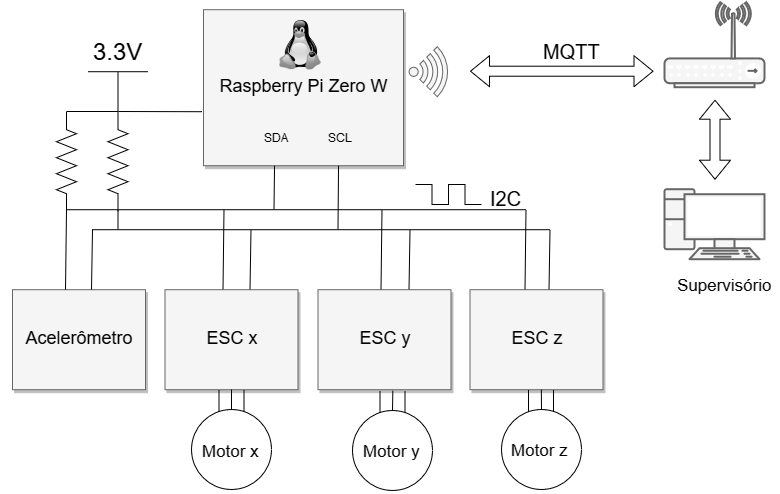
\includegraphics[scale=.75]{img/comunicacao_projeto}
  \end{center}
  \fonte{Elaborado peloAutor.} 
  \label{fig:pid_neural_Applying_p18}
\end{figure}

%%%%%%%%%%%%%%%%%%%%%%%%%%%%%%%%%%%
\subsection{Rodas de Reação e Motores}

%%%%%%%%%%%%%%%%%%%%%%%%%%%%%%%%%%%
\subsection{Sistema Embarcado}

%%%%%%%%%%%%%%%%%%%%%%%%%%%%%%%%%%%%%%%%%%%%%%%%%%%%%%%%%%%%%%%%%%%%%%
\section{Software}

%%%%%%%%%%%%%%%%%%%%%%%%%%%%%%%%%%%
\subsection{Protocolos de Comunicação}
\subsubsection{Protocolos de MQTT e I2C}

%%%%%%%%%%%%%%%%%%%%%%%%%%%%%%%%%%%
\subsection{Implementação do Controlador PID}

%%%%%%%%%%%%%%%%%%%%%%%%%%%%%%%%%%%
\subsection{Implementação da Rede Neural}

%%%%%%%%%%%%%%%%%%%%%%%%%%%%%%%%%%%
\subsection{Sistemas Supervisórios}
